\documentclass{article}

\usepackage{amsmath}
\usepackage{graphicx}

\graphicspath{ {./assets/} }

\setlength\paperwidth{20.999cm}\setlength\paperheight{29.699cm}\setlength\voffset{-1in}\setlength\hoffset{-1in}\setlength\topmargin{1.499cm}\setlength\headheight{12pt}\setlength\headsep{0cm}\setlength\footskip{1.131cm}\setlength\textheight{25cm}\setlength\oddsidemargin{2.499cm}\setlength\textwidth{15.999cm}

\begin{document}
\begin{center}
\hrule

\vspace{.4cm}
{\bf {\Huge Assignment 4}} \\
\vspace{.2cm}
{\bf Computer Graphics}
\vspace{.2cm}
\end{center}{\bf Edoardo Riggio } (edoardo.riggio@usi.ch) \hspace{\fill}  \today \\
\hrule
\vspace{.2cm}

\section{Exercise 1}
\subsection{Task 1}
The two matrices $R_{90}$ and $T$ in homogeneous coordinates are as follows.
\[ R_{90} = \begin{bmatrix} 1 & 0 & 1 \\ 0 & 1 & -2 \\ 0 & 0 & 1 \end{bmatrix} \]
\[ T = \begin{bmatrix} \cos{90} & -\sin{90} & 0 \\ \sin{90} & \cos{90} & 0 \\ 0 & 0 & 1 \end{bmatrix} = \begin{bmatrix} 0 & -1 & 0 \\ 1 & 0 & 0 \\ 0 & 0 & 1 \end{bmatrix} \]

\subsection{Task 2}
The following are the computations for the rotated and translated points and vector.
\begin{align*}
	p'_1 & =  \begin{bmatrix}1&0&1\\ 0&1&-2\\0&0&1\end{bmatrix} \left( \begin{bmatrix}0&-1&0\\ 1&0&0\\ 0&0&1\end{bmatrix}\begin{bmatrix}1\\ 1\\ 1\end{bmatrix} \right)  =  \begin{bmatrix}1&0&1\\ 0&1&-2\\0&0&1\end{bmatrix}\begin{bmatrix}0\cdot 1+\left(-1\right)\cdot 1+0\cdot 1\\ 1\cdot 1+0\cdot 1+0\cdot 1\\ 0\cdot 1+0\cdot 1+1\cdot 1\end{bmatrix} \\
	& = \begin{bmatrix}1&0&1\\ 0&1&-2\\0&0&1\end{bmatrix}\begin{bmatrix}-1\\ 1\\ 1\end{bmatrix} = \begin{bmatrix}1\cdot \left(-1\right)+0\cdot 1+1\cdot 1\\ 0\cdot \left(-1\right)+1\cdot 1+\left(-2\right)\cdot 1\\ 0\cdot \left(-1\right)+0\cdot 1+1\cdot 1\end{bmatrix} = \begin{bmatrix}0\\ -1\\ 1\end{bmatrix} \mapsto \begin{bmatrix}0\\ -1\end{bmatrix}
\end{align*}

\begin{align*}
	p'_2 & =  \begin{bmatrix}1&0&1\\ 0&1&-2\\0&0&1\end{bmatrix} \left( \begin{bmatrix}0&-1&0\\ 1&0&0\\ 0&0&1\end{bmatrix}\begin{bmatrix}3\\ 2\\ 1\end{bmatrix} \right)  =  \begin{bmatrix}1&0&1\\ 0&1&-2\\0&0&1\end{bmatrix}\begin{bmatrix}0\cdot 3+\left(-1\right)\cdot 2+0\cdot 1\\ 1\cdot 3+0\cdot 2+0\cdot 1\\ 0\cdot 3+0\cdot 2+1\cdot 1\end{bmatrix} \\
	& = \begin{bmatrix}1&0&1\\ 0&1&-2\\0&0&1\end{bmatrix}\begin{bmatrix}-2\\ 3\\ 1\end{bmatrix} = \begin{bmatrix}1\cdot \left(-2\right)+0\cdot 3+1\cdot 1\\ 0\cdot \left(-2\right)+1\cdot 3+\left(-2\right)\cdot 1\\ 0\cdot \left(-2\right)+0\cdot 3+1\cdot 1\end{bmatrix} = \begin{bmatrix}-1\\ 1\\ 1\end{bmatrix} \mapsto \begin{bmatrix}-1\\ 1\end{bmatrix}
\end{align*}

\begin{align*}
	p'_2 & =  \begin{bmatrix}1&0&1\\ 0&1&-2\\0&0&1\end{bmatrix} \left( \begin{bmatrix}0&-1&0\\ 1&0&0\\ 0&0&1\end{bmatrix}\begin{bmatrix}1\\ 4\\ 1\end{bmatrix} \right)  =  \begin{bmatrix}1&0&1\\ 0&1&-2\\0&0&1\end{bmatrix}\begin{bmatrix}0\cdot 1+\left(-1\right)\cdot 4+0\cdot 1\\ 1\cdot 1+0\cdot 4+0\cdot 1\\ 0\cdot 1+0\cdot 4+1\cdot 1\end{bmatrix} \\
	& = \begin{bmatrix}1&0&1\\ 0&1&-2\\0&0&1\end{bmatrix}\begin{bmatrix}-4\\ 1\\ 1\end{bmatrix} = \begin{bmatrix}1\cdot \left(-4\right)+0\cdot 1+1\cdot 1\\ 0\cdot \left(-4\right)+1\cdot 1+\left(-2\right)\cdot 1\\ 0\cdot \left(-4\right)+0\cdot 1+1\cdot 1\end{bmatrix} = \begin{bmatrix}-3\\ -1\\ 1\end{bmatrix} \mapsto \begin{bmatrix}-3\\ -1\end{bmatrix}
\end{align*}

\begin{align*}
	p' & =  \begin{bmatrix}1&0&1\\ 0&1&-2\\0&0&1\end{bmatrix} \left( \begin{bmatrix}0&-1&0\\ 1&0&0\\ 0&0&1\end{bmatrix}\begin{bmatrix}1.5\\ 2.5\\ 1\end{bmatrix} \right)  =  \begin{bmatrix}1&0&1\\ 0&1&-2\\0&0&1\end{bmatrix}\begin{bmatrix}0\cdot 1.5+\left(-1\right)\cdot 2.5+0\cdot 1\\ 1\cdot 1.5+0\cdot 2.5+0\cdot 1\\ 0\cdot 1.5+0\cdot 2.5+1\cdot 1\end{bmatrix} \\
	& = \begin{bmatrix}1&0&1\\ 0&1&-2\\0&0&1\end{bmatrix}\begin{bmatrix}-2.5\\ 1.5\\ 1\end{bmatrix} = \begin{bmatrix}1\cdot \left(-2.5\right)+0\cdot 1.5+1\cdot 1\\ 0\cdot \left(-2.5\right)+1\cdot 1.5+\left(-2\right)\cdot 1\\ 0\cdot \left(-2.5\right)+0\cdot 1.5+1\cdot 1\end{bmatrix} = \begin{bmatrix}-1.5\\ -0.5\\ 1\end{bmatrix} \mapsto \begin{bmatrix}-1.5\\ -0.5 \end{bmatrix}
\end{align*}

\begin{align*}
	u' & =  \begin{bmatrix}1&0&1\\ 0&1&-2\\0&0&1\end{bmatrix} \left( \begin{bmatrix}0&-1&0\\ 1&0&0\\ 0&0&1\end{bmatrix}\begin{bmatrix}0.5\\ 1.5\\ 0\end{bmatrix} \right)  =  \begin{bmatrix}1&0&1\\ 0&1&-2\\0&0&1\end{bmatrix}\begin{bmatrix}0\cdot 0.5+\left(-1\right)\cdot 1.5+0\cdot 0\\ 1\cdot 0.5+0\cdot 1.5+0\cdot 0\\ 0\cdot 0.5+0\cdot 1.5+1\cdot 0\end{bmatrix} \\
	& = \begin{bmatrix}1&0&1\\ 0&1&-2\\0&0&1\end{bmatrix}\begin{bmatrix}-1.5\\ 0.5\\ 0\end{bmatrix} = \begin{bmatrix}1\cdot \left(-1.5\right)+0\cdot 0.5+1\cdot 0\\ 0\cdot \left(-1.5\right)+1\cdot 0.5+\left(-2\right)\cdot 0\\ 0\cdot \left(-1.5\right)+0\cdot 0.5+1\cdot 0\end{bmatrix} = \begin{bmatrix}-1.5\\ 0.5\\ 0\end{bmatrix} \mapsto \begin{bmatrix}-1.5\\ 0.5 \end{bmatrix}
\end{align*}
Now we can see that $u' = p' - p'_1$, as shown below:
\[ \begin{bmatrix}-1.5\\ 0.5\\ 0\end{bmatrix} = \begin{bmatrix}-1.5\\ -0.5\\ 1\end{bmatrix} - \begin{bmatrix}0\\ -1\\ 1\end{bmatrix} = \begin{bmatrix}-1.5\\ 0.5\\ 0\end{bmatrix} \]
The translation only works with points, while the rotation works with both points and vectors. For this reason, the vector $u'$ is only affected by the rotation matrix, and not by the translation matrix. \\ \\
Finally, here is a visual representation of all the points and vector before and after the transformations. \\

\begin{center}
	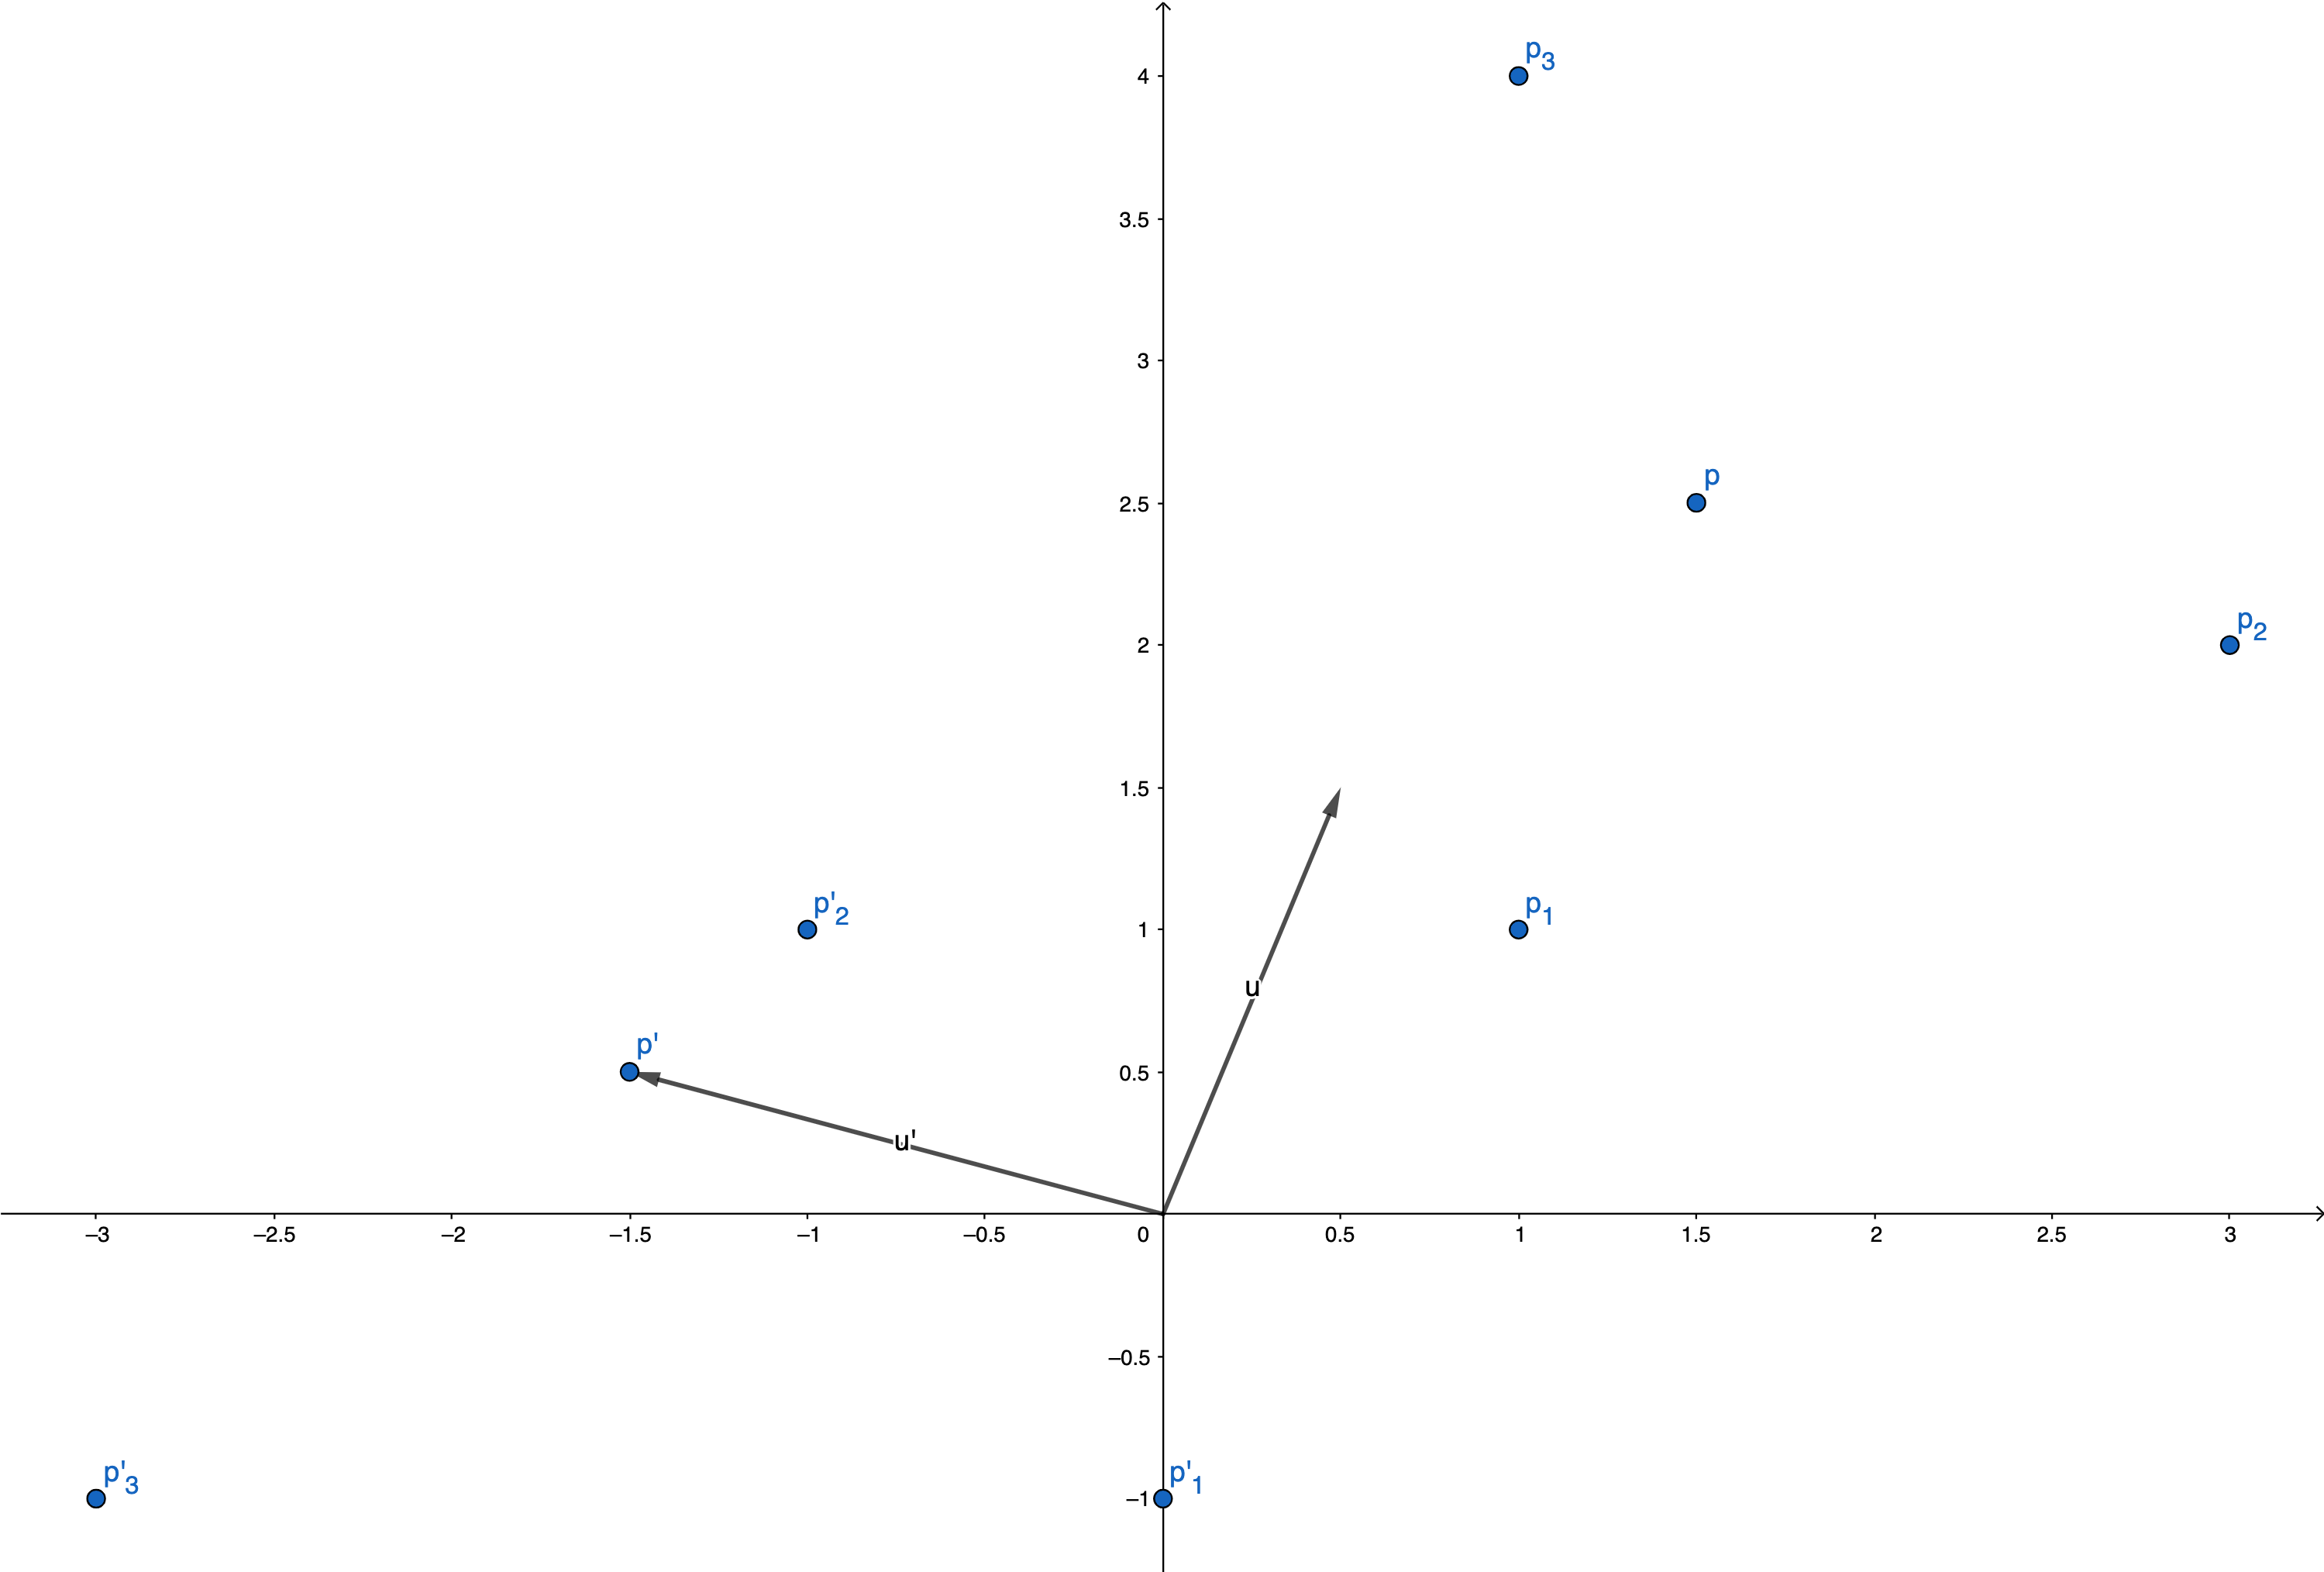
\includegraphics[width=15cm]{task_2.png}
\end{center}

\subsection{Task 3}
Here we have the scaling matrix which scales both $x$ and $y$ by a factor of 2.
\[ S = \begin{bmatrix} 2 & 0 & 0 \\ 0 & 2 & 0 \\ 0 & 0 & 1 \end{bmatrix} \]
The following are the computations for the scaled points and vector.

\begin{align*}
	p''_1 = \begin{bmatrix}2&0&0\\ 0&2&0\\ 0&0&1\end{bmatrix}\begin{bmatrix}0\\ -1\\ 1\end{bmatrix} = \begin{bmatrix}2\cdot 0+0\cdot \left(-1\right)+0\cdot 1\\ 0\cdot 0+2\left(-1\right)+0\cdot 1\\ 0\cdot 0+0\cdot \left(-1\right)+1\cdot 1\end{bmatrix} = \begin{bmatrix}0\\ -2\\ 1\end{bmatrix} \mapsto \begin{bmatrix}0\\ -2\end{bmatrix}
\end{align*}

\begin{align*}
	p''_2 = \begin{bmatrix}2&0&0\\ 0&2&0\\ 0&0&1\end{bmatrix}\begin{bmatrix}-1\\ 1\\ 1\end{bmatrix} = \begin{bmatrix}2\left(-1\right)+0\cdot 1+0\cdot 1\\ 0\cdot \left(-1\right)+2\cdot 1+0\cdot 1\\ 0\cdot \left(-1\right)+0\cdot 1+1\cdot 1\end{bmatrix} = \begin{bmatrix}-2\\ 2\\ 1\end{bmatrix} \mapsto \begin{bmatrix}-2\\ 2\end{bmatrix}
\end{align*}

\begin{align*}
	p''_3 = \begin{bmatrix}2&0&0\\ 0&2&0\\ 0&0&1\end{bmatrix}\begin{bmatrix}-3\\ -1\\ 1\end{bmatrix} = \begin{bmatrix}2\left(-3\right)+0\cdot \left(-1\right)+0\cdot 1\\ 0\cdot \left(-3\right)+2\left(-1\right)+0\cdot 1\\ 0\cdot \left(-3\right)+0\cdot \left(-1\right)+1\cdot 1\end{bmatrix} = \begin{bmatrix}-6\\ -2\\ 1\end{bmatrix} \mapsto \begin{bmatrix}-6\\ -2\end{bmatrix}
\end{align*}

\begin{align*}
	p'' = \begin{bmatrix}2&0&0\\ 0&2&0\\ 0&0&1\end{bmatrix}\begin{bmatrix}-1.5\\ -0.5\\ 1\end{bmatrix} = \begin{bmatrix}2\left(-1.5\right)+0\cdot \left(-0.5\right)+0\cdot 1\\ 0\cdot \left(-1.5\right)+2\left(-0.5\right)+0\cdot 1\\ 0\cdot \left(-1.5\right)+0\cdot \left(-0.5\right)+1\cdot 1\end{bmatrix} = \begin{bmatrix}-3\\ -1\\ 1\end{bmatrix} \mapsto \begin{bmatrix}-3\\ -1\end{bmatrix}
\end{align*}

\begin{align*}
	u'' = \begin{bmatrix}2&0&0\\ 0&2&0\\ 0&0&1\end{bmatrix}\begin{bmatrix}-1.5\\ 0.5\\ 0\end{bmatrix} = \begin{bmatrix}2\left(-1.5\right)+0\cdot 0.5+0\cdot 0\\ 0\cdot \left(-1.5\right)+2\cdot 0.5+0\cdot 0\\ 0\cdot \left(-1.5\right)+0\cdot 0.5+1\cdot 0\end{bmatrix} = \begin{bmatrix}-3\\ 1\\ 0\end{bmatrix} \mapsto \begin{bmatrix}-3\\ 1\end{bmatrix}
\end{align*}
Finally, here is a visual representation of the points and the vector before and after the scaling. \\

\begin{center}
	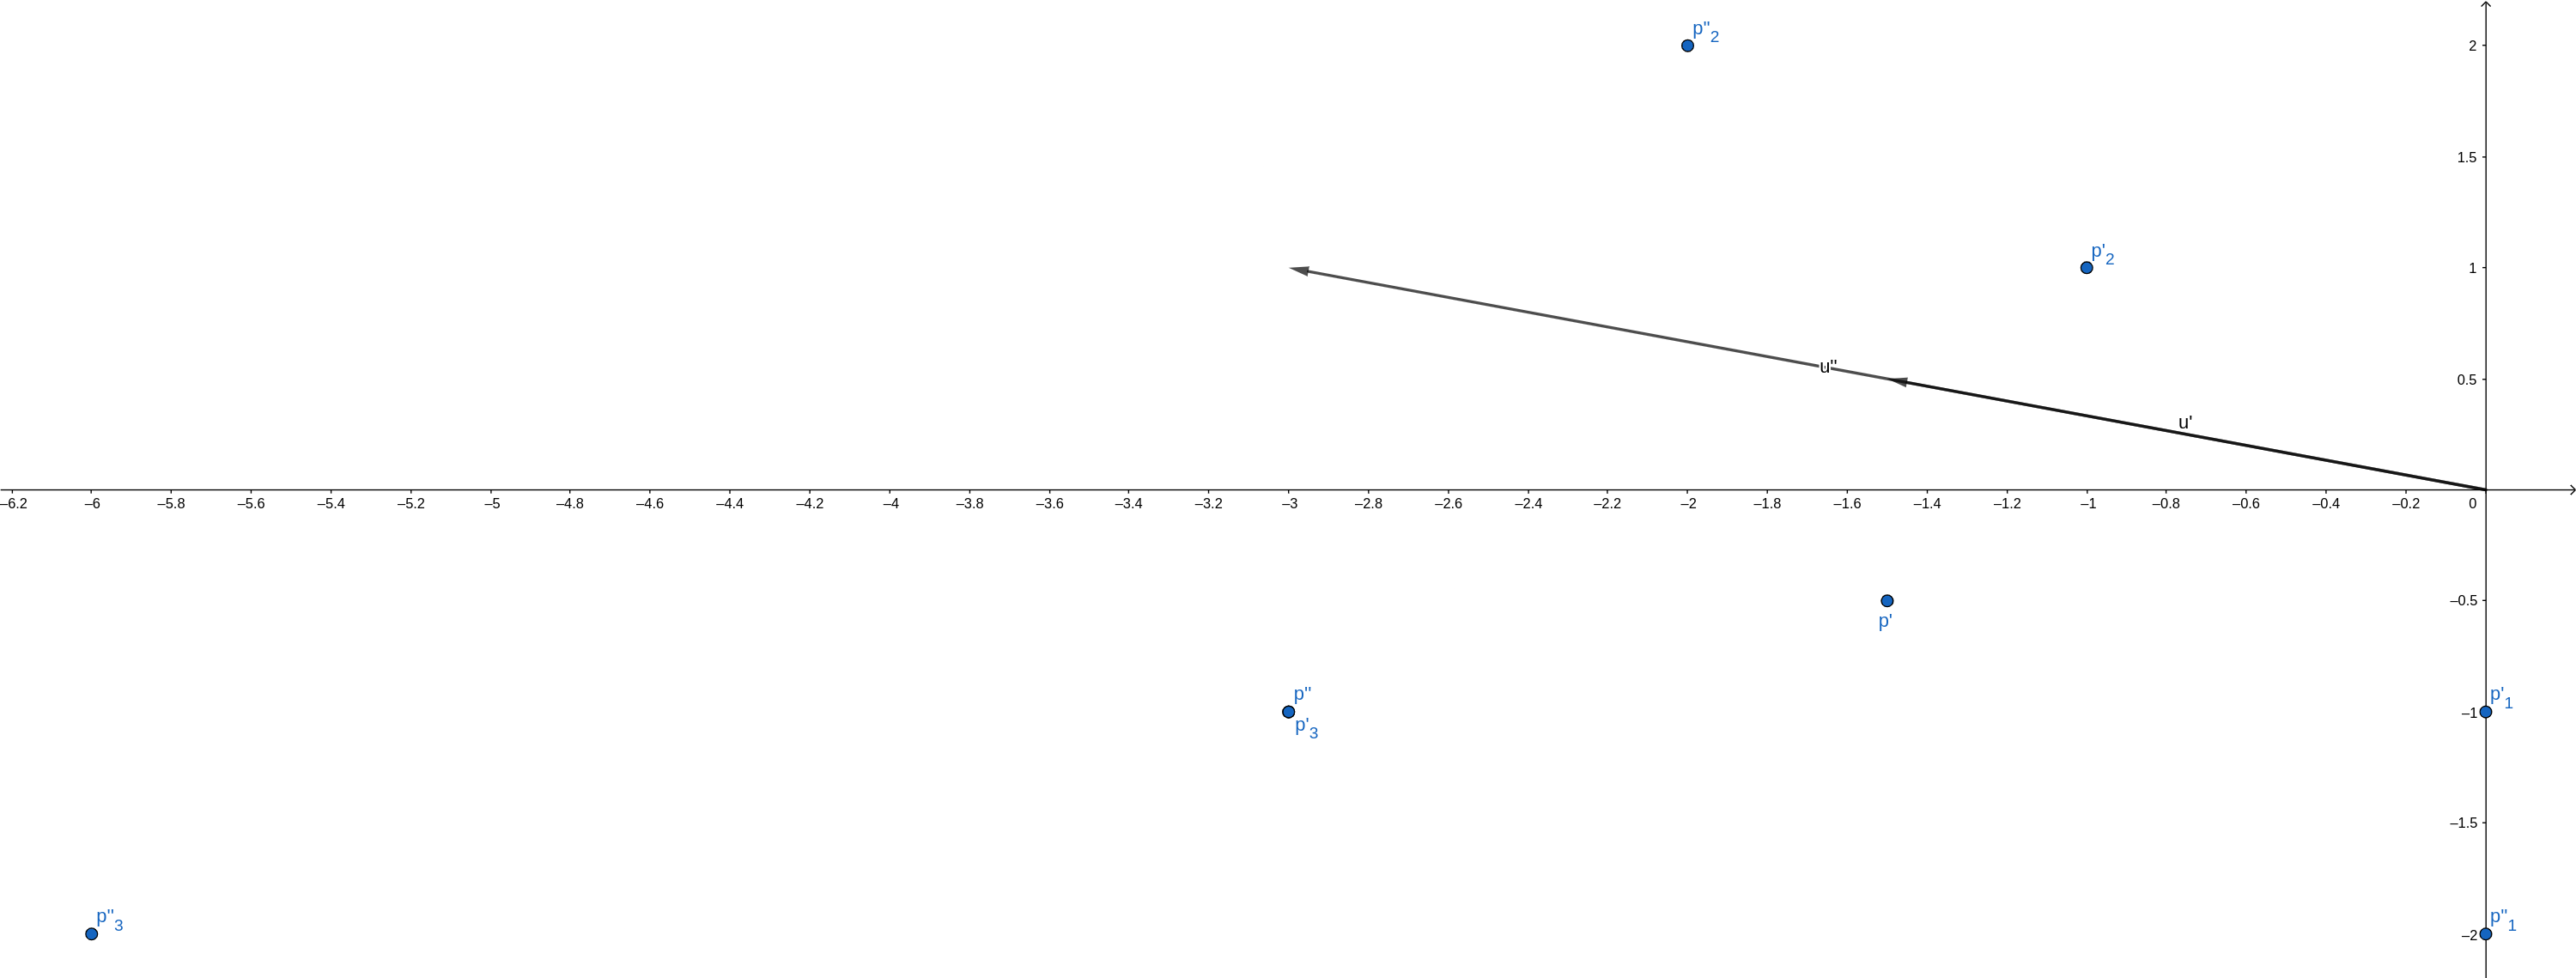
\includegraphics[width=15cm]{task_3.png}
\end{center}

\subsection{Task 4}
In order to apply the inverse transformations, we need to compute the inverse matrices for rotation, translation and scaling.
\[ R_{90}^{-1} = \begin{bmatrix} 0 & 1 & 0 \\ -1 & 0 & 0 \\ 0 & 0 & 1 \end{bmatrix} \]
\[ T^{-1} = \begin{bmatrix} 1 & 0 & -1 \\ 0 & 1 & 2 \\ 0 & 0 & 1 \end{bmatrix} \]
\[ S^{-1} = \begin{bmatrix} 0.5 & 0 & 0 \\ 0 & 0.5 & 0 \\ 0 & 0 & 1 \end{bmatrix} \]
And we compute the transformation matrix $M$.

\begin{align*}
	M & = R_{90}^{-1} T^{-1} S^{-1} = \begin{bmatrix} 0 & 1 & 0 \\ -1 & 0 & 0 \\ 0 & 0 & 1 \end{bmatrix} \begin{bmatrix} 1 & 0 & -1 \\ 0 & 1 & 2 \\ 0 & 0 & 1 \end{bmatrix} \begin{bmatrix} 0.5 & 0 & 0 \\ 0 & 0.5 & 0 \\ 0 & 0 & 1 \end{bmatrix} \\ 
	& = \begin{bmatrix}0\cdot 1+1\cdot 0+0\cdot 0&0\cdot 0+1\cdot 1+0\cdot 0&0\cdot \left(-1\right)+1\cdot 2+0\cdot 1\\ \left(-1\right)\cdot 1+0\cdot 0+0\cdot 0&\left(-1\right)\cdot 0+0\cdot 1+0\cdot 0&\left(-1\right)\left(-1\right)+0\cdot 2+0\cdot 1\\ 0\cdot 1+0\cdot 0+1\cdot 0&0\cdot 0+0\cdot 1+1\cdot 0&0\cdot \left(-1\right)+0\cdot 2+1\cdot 1\end{bmatrix} \begin{bmatrix} 0.5 & 0 & 0 \\ 0 & 0.5 & 0 \\ 0 & 0 & 1 \end{bmatrix} \\
	& = \begin{bmatrix}0&1&2\\ -1&0&1\\ 0&0&1\end{bmatrix} \begin{bmatrix} 0.5 & 0 & 0 \\ 0 & 0.5 & 0 \\ 0 & 0 & 1 \end{bmatrix} \\
	& = \begin{bmatrix}0\cdot 0.5+1\cdot 0+2\cdot 0&0\cdot 0+1\cdot 0.5+2\cdot 0&0\cdot 0+1\cdot 0+2\cdot 1\\ \left(-1\right)\cdot 0.5+0\cdot 0+1\cdot 0&\left(-1\right)\cdot 0+0\cdot 0.5+1\cdot 0&\left(-1\right)\cdot 0+0\cdot 0+1\cdot 1\\ 0\cdot 0.5+0\cdot 0+1\cdot 0&0\cdot 0+0\cdot 0.5+1\cdot 0&0\cdot 0+0\cdot 0+1\cdot 1\end{bmatrix} = \begin{bmatrix}0&0.5&2\\ -0.5&0&1\\ 0&0&1\end{bmatrix}
\end{align*}

\pagebreak
\noindent Now that we have the transformation matrix $M$, we can finally compute the transformation of points $p_1''$, $p_2''$, $p_3''$, $p''$ and of vector $u''$.

\begin{align*}
	p_1 & = \begin{bmatrix}0&0.5&2\\ -0.5&0&1\\ 0&0&1\end{bmatrix} \begin{bmatrix}0\\ -2\\ 1\end{bmatrix} = \begin{bmatrix}0\cdot 0+0.5\left(-2\right)+2\cdot 1\\ \left(-0.5\right)\cdot 0+0\cdot \left(-2\right)+1\cdot 1\\ 0\cdot 0+0\cdot \left(-2\right)+1\cdot 1\end{bmatrix} = \begin{bmatrix}1\\ 1\\ 1\end{bmatrix}
\end{align*}

\begin{align*}
	p_2 & = \begin{bmatrix}0&0.5&2\\ -0.5&0&1\\ 0&0&1\end{bmatrix} \begin{bmatrix}-2\\ 2\\ 1\end{bmatrix} = \begin{bmatrix}0\cdot \left(-2\right)+0.5\cdot 2+2\cdot 1\\ \left(-0.5\right)\left(-2\right)+0\cdot 2+1\cdot 1\\ 0\cdot \left(-2\right)+0\cdot 2+1\cdot 1\end{bmatrix} = \begin{bmatrix}3\\ 2\\ 1\end{bmatrix}
\end{align*}

\begin{align*}
	p_2 & = \begin{bmatrix}0&0.5&2\\ -0.5&0&1\\ 0&0&1\end{bmatrix} \begin{bmatrix}-6\\ -2\\ 1\end{bmatrix} = \begin{bmatrix}0\cdot \left(-6\right)+0.5\left(-2\right)+2\cdot 1\\ \left(-0.5\right)\left(-6\right)+0\cdot \left(-2\right)+1\cdot 1\\ 0\cdot \left(-6\right)+0\cdot \left(-2\right)+1\cdot 1\end{bmatrix} = \begin{bmatrix}1\\ 4\\ 1\end{bmatrix}
\end{align*}

\begin{align*}
	p & = \begin{bmatrix}0&0.5&2\\ -0.5&0&1\\ 0&0&1\end{bmatrix} \begin{bmatrix}-3\\ -1\\ 1\end{bmatrix} = \begin{bmatrix}0\cdot \left(-3\right)+0.5\left(-1\right)+2\cdot 1\\ \left(-0.5\right)\left(-3\right)+0\cdot \left(-1\right)+1\cdot 1\\ 0\cdot \left(-3\right)+0\cdot \left(-1\right)+1\cdot 1\end{bmatrix} = \begin{bmatrix}1.5\\ 2.5\\ 1\end{bmatrix}
\end{align*}

\begin{align*}
	u & = \begin{bmatrix}0&0.5&2\\ -0.5&0&1\\ 0&0&1\end{bmatrix} \begin{bmatrix}-3\\ 1\\ 0\end{bmatrix} = \begin{bmatrix}0\cdot \left(-3\right)+0.5\cdot 1+2\cdot 0\\ \left(-0.5\right)\left(-3\right)+0\cdot 1+1\cdot 0\\ 0\cdot \left(-3\right)+0\cdot 1+1\cdot 0\end{bmatrix} = \begin{bmatrix}0.5\\ 1.5\\ 0\end{bmatrix}
\end{align*}
As we can see, by multiplying the transformation matrix with $p_1''$, $p_2''$, $p_3''$, $p''$ and $u''$, we will get back $p_1$, $p_2$, $p_3$, $p$ and $u$.

\end{document}


















